\chapter{Back-end design}
This chapter describes the communication between server and client, aswell as the design choices and
implementation of database. \todo{Bør database være et kapitel for sig selv?}

\section{Communication}
\label{sec:com}

The communication betweeen the client application and the server is done by HTTP POST requests.
The client sends a HTTP POST request to the server containing a certain list of parameters which
define what the server is supposed to do. All requests must take atleast two required parameters, a \textit{RequestCode} and a
\textit{Type}.

\textit{RequestCode} is an integer that is simply passed through the server, it is not handled in any
way on the server. The purpose of the RequestCode parameter is to distinguish the request on the client allowing
it to execute the appropriate function.

\textit{Type} is used to identify the request. A typical request is to get a list of feeds, and the
value of the \textit{Type} parameter would be ``GetFeeds'' in this case.\\

Depending on the \textit{Type} of the request, additional parameters may be required.\\

As an example, \textit{GetFeeds} takes the following parameters:
\begin{itemize}
\item RequestCode
\item UserId
\item Limit
\end{itemize}

The approach is to process the request on the serverside, and make the right calls to the
database. The server will then return a JSON object containing all the relevant information that was
requested. This JSON object can easily be parsed on the client side. The reason why we chose JSON as
a format is because it is well supported and easy to generate in both android and PHP.

\begin{lstlisting}[language=phpstyle, caption=getFeeds function call]
$requestCode = $_POST["RequestCode"];

switch ($_POST['Type']) {
        case "GetFeeds":
            getFeeds($con, $_POST['UserId'], $_POST['Limit']);
            break;
}
\end{lstlisting}

\begin{description}
\item \textbf{Line 1: }Get the \textit{RequestCode} parameter.
\item \textbf{Lines 3-7: }If \textit{Type} equals ``GetFeeds'', call the getFeeds function.
\end{description}

\todo{Nævn de andre cases, måske her?}

\begin{lstlisting}[language=phpstyle, label=lst:getFeeds, caption=getFeeds function]
function getFeeds($con, $userId, $limit) {

    global $requestCode;

    #Escape special characters to avoid SQL injection attacks
    $userId    = $con->real_escape_string($userId);
    $limit     = $con->real_escape_string($limit);

    $query =   "SELECT feeds.id, feeds.boothid, feeds.header, feeds.description, feeds.feedtime, userbooths.userid, companies.logo, booths.name ".
        "FROM feeds ".
        "LEFT JOIN userbooths ".
        "ON feeds.boothid = userbooths.boothid ".
        "LEFT JOIN booths ".
        "ON feeds.boothid = booths.id ".
        "LEFT JOIN companies ".
        "ON booths.companyid = companies.id ".
        "WHERE userid = ".$userId." ".
        "AND sub = 1 ".
        "ORDER BY feeds.feedtime DESC ".
        "LIMIT "$limit;

    $result = $con->query($query);

    $json = array();
    while($row = $result->fetch_object()) {
      array_push($json, $row);
    }
    echo $requestCode;
    echo json_encode($json);
}
\end{lstlisting}%$

\begin{description}
\item[Line 1] The function takes three parameters, the MySQLi object which has a connection
  established to the database, the user id from the client, and the limit which is also given by the client.
\item[Line 3] Since the \textit{RequestCode} is always a required parameter the variable is global.
\item[Lines 6-7] Escape special characters to avoid malicious SQL injections.
\item[Lines 9-20] Create the SQL query with the user id and the limit paramter.
\item[Line 22] Execute the query.
\item[Lines 24-29] Get the results from the database and push them to the JSON array. When
  all of the results have been pushed to the array, the \textit{RequestCode} will be echoed and then
  a JSON encoded version of the array.
\end{description}

As seen on line 29 in \autoref{lst:getFeeds} the result is JSON encoded and then echoed. An example of a result from the \textit{GetFeeds} type request could look like the following:

\begin{lstlisting}[language=json, label=lst:jsonResult, caption=Example result from a request with type: \textit{GetFeeds}]
1[
    {
        "id": "18",
        "boothid": "2",
        "header": "asdf",
        "description": "Super.",
        "feedtime": "2013-10-02 12:41:02",
        "userid": "1",
        "logo": "microsoftlogo.png",
        "name": "Microsoft XBOX"
    },
    {
        "id": "17",
        "boothid": "2",
        "header": "short header",
        "description": "short description.",
        "feedtime": "2013-10-02 11:43:28",
        "userid": "1",
        "logo": "microsoftlogo.png",
        "name": "Microsoft XBOX"
    }
]
\end{lstlisting}

Note the number before the array in \autoref{lst:jsonResult}, this is the request code.

All of the requests to the server follows this principle. A request is made, the query is run and data is gathered, and lastly the result is returned as a JSON object that the client reads.\\\\
Our types of requests are as follows:
\begin{itemize}
\item \textbf{GetFeeds}\\
 Will return all the necessary data about a certain number of feeds. They are sorted to return the newest feed first and then the next number of feeds that coresponds to the given limit parameter.
\item \textbf{CreateUser}\\
  Creates a new user in the database and returns the userid.
\item \textbf{GetNewFeeds}\\
  Returns data about all new feeds since the last update. This means that the user can manually fetch all new feeds.
\item \textbf{CheckFeeds}\\
  Check if any new feeds are available, and if such the number of new feeds will be returned.
\item \textbf{GetOldFeeds}\\
  Load a certain number of feeds that are older than the current oldest feed showing. This allows the user to load the next batch of feeds.
\item \textbf{GetSchedule}\\
  Returns relevant data about the schedule of the exhibition. Used for the schedule tab on the android application.
\item \textbf{GetExhibitionInfo}\\
  Returns all information about the exhibition, such as the description and logo.
\item \textbf{GetCategories}\\
  Returns a list of categories, and the booths of this category, that are associated with the current exhibition. It also contains a flag that shows whether the user is currently subscribed to a booth or not.
\item \textbf{SetCategories}\\
  This request is run when the ``submit'' button is pressed in the category chooser. This updates the booths that the user is subscribed to in the databse.
\end{itemize}

\section{Database}
We are using a MySQL database with the MyISAM storage engine and which is located at a remote server. \todo{info om hvor osv.?}

The server is to contain all data about each exhibition, the companies at the exhibition, the feeds, the schedule, and some basic information about the users.

\begin{figure}[H]
\centering
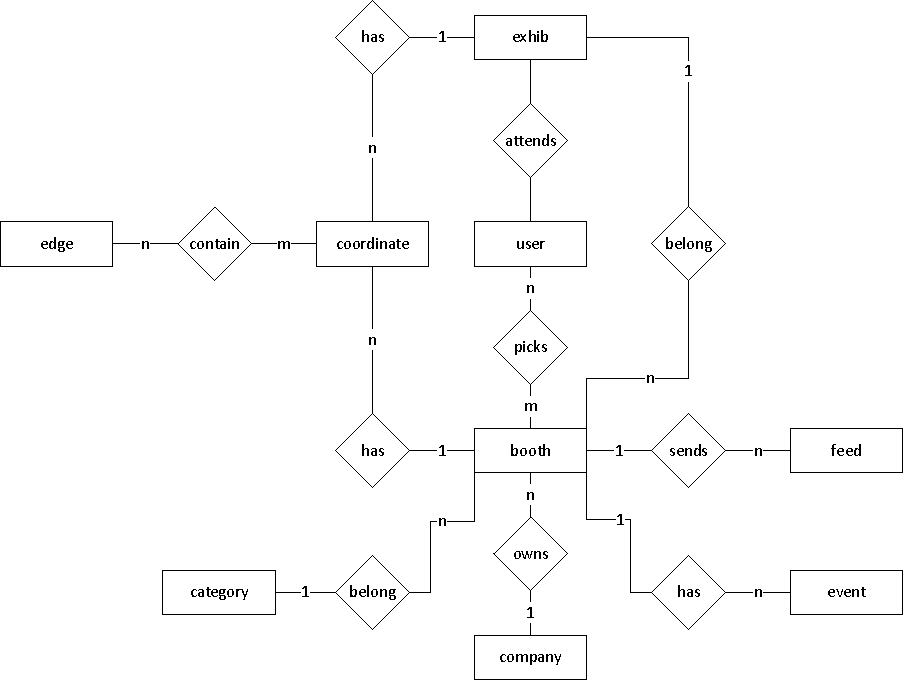
\includegraphics[page=1,width=1\linewidth]{img/sw7ERD.pdf}
\caption{Entity-relation diagram}
\label{fig:erd}
\end{figure}
\todo{ERD skal opdateres!!}

%%% Local Variables: 
%%% mode: latex
%%% TeX-master: "../master"
%%% End: 
